\documentclass[10pt,a4paper]{article}
\usepackage[utf8]{inputenc}

% \usepackage{ngerman}  % german documents
\usepackage{graphicx}  % import graphics einbinden
\usepackage{listings}  % support source code listing
\usepackage{amsmath}  % math stuff
\usepackage{amssymb} % 
\usepackage{a4wide} % wide pages
\usepackage{fancyhdr} % nice headers
\usepackage{float}
\usepackage{longtable}
\usepackage{xcolor}
\usepackage{booktabs}
\definecolor{darkpastelgreen}{rgb}{0.01, 0.75, 0.24}
\definecolor{spirodiscoball}{rgb}{0.06, 0.75, 0.99}
\definecolor{smalt}{rgb}{0.0, 0.2, 0.6}
\definecolor{armygreen}{rgb}{0.29, 0.33, 0.13}
\definecolor{awesome}{rgb}{1.0, 0.13, 0.32}
\definecolor{bittersweet}{rgb}{1.0, 0.44, 0.37}
\definecolor{bananayellow}{rgb}{1.0, 0.88, 0.21}
\definecolor{blue}{rgb}{0.0, 0.0, 1.0}
\definecolor{red}{rgb}{1.0, 0.0, 0.0}
\definecolor{green}{rgb}{0.0, 1.0, 0.0}



\lstset{basicstyle=\footnotesize,language=Python,breaklines=true,numbers=left, numberstyle=\tiny, stepnumber=5,firstnumber=0, numbersep=5pt} % set up listings
\pagestyle{fancy}             % header
\setlength{\parindent}{0pt}   % no indentation
 

\usepackage[pdfpagemode=None, colorlinks=true,  % url coloring
           linkcolor=blue, urlcolor=blue, citecolor=blue, plainpages=false, 
           pdfpagelabels,unicode]{hyperref}
           
% change enums style: first level (a), (b), (c)           
\renewcommand{\labelenumi}{(\alph{enumi})}
\renewcommand{\labelenumii}{(\arabic{enumii})}

\newcommand{\norm}[1]{\left\lVert#1\right\rVert}

%lecture name
\newcommand{\lecture}{
	Bioinformatics III
}           

%assignment iteration
\newcommand{\assignment}{
	Sixth Assignment
}


%set up names, matricle number, and email
\newcommand{\authors}{
  \begin{tabular}{rl}
    \href{mailto:s8tbscho@stud.uni-saarland.de}{Thibault Schowing} & (2571837)\\
    \href{mailto:wiebkeschmitt@outlook.de}{Wiebke Schmitt} & (2543675)
  \end{tabular}
}

% use to start a new exercise
\newcommand{\exercise}[1]
{
  \stepcounter{subsection}
  \subsection*{Exercise \thesubsection: #1}

}

\begin{document}
\title{\Large \lecture \\ \textbf{\normalsize \assignment}}
\author{\authors}

\setlength \headheight{25pt}
\fancyhead[R]{\begin{tabular}{r}\lecture \\ \assignment \end{tabular}}
\fancyhead[L]{\authors}


\setcounter{section}{6} % modify for later sheets, i.e. 2, 3, ...
%\section{Introduction to Python and some Network Properties} % optional, note that section invocation sets the section counter + 1, so adapt the setcounter command
\maketitle

%EXERCICE 1
\exercise{Boolean Networks}
All the listings are at the end of the exercise. 
\begin{enumerate}

% A
\item \textbf{Weighted Interactions}\\ 

\begin{table}[H]
	\centering
	\caption{Propagation Matrix }
	\label{my-label}
	\begin{tabular}{l|l|l|l|l|l|l|}
		\cline{2-7}
		& F  & E  & D & C & B  & A \\ \hline
		\multicolumn{1}{|l|}{F} & 0  & 0  & 1 & 0 & 0  & 0 \\ \hline
		\multicolumn{1}{|l|}{E} & 1  & 0  & 0 & 0 & 0  & 0 \\ \hline
		\multicolumn{1}{|l|}{D} & -3 & -3 & 0 & 0 & -3 & 0 \\ \hline
		\multicolumn{1}{|l|}{C} & 0  & 1  & 0 & 0 & 1  & 0 \\ \hline
		\multicolumn{1}{|l|}{B} & 0  & 0  & 0 & 1 & 0  & 0 \\ \hline
		\multicolumn{1}{|l|}{A} & 0  & 0  & 0 & 0 & 1  & 1 \\ \hline
	\end{tabular}
\end{table}


% B
\item \textbf{Implementation}\\

\textit{When does it make sense to stop the propagation and why?}\\

We stop the propagation once we meet an already visited state. If we continue, we will just loop over and over again.\\


\textit{Which sequences do you get when you start from states 1, 4, 21, and 33?}\\

Sequence with starting state 1:  [1, 3, 7, 23, 55, 63, 13, 1]\\
Sequence with starting state 4:  [4, 18, 36, 26, 4]\\
Sequence with starting state 21: [21, 51, 47, 13, 1, 3, 7, 23, 55, 63, 13]\\
Sequence with starting state 33: [33, 11, 5, 19, 39, 31, 5]\\





% C
\newpage
\item \textbf{Periodic Orbits}\\
\textbf{\textit{(1) List these orbits with their respective lengths and basins of attraction}}\\

To make things clearer let's recall the different definition. "If the attractor has only a single state it is called a point attractor, and if the attractor consists of more than one state it is called a cycle attractor. The set of states that lead to an attractor is called the basin of the attractor. States which occur only at the beginning of trajectories (no trajectories lead to them), are called garden-of-Eden states" \footnote{\url{https://en.wikipedia.org/wiki/Boolean\string_network\#Attractors}}\\




\begin{table}[H]
	\centering
	\caption{List of states, orbith length, Cycle attractor and relative coverage of the basin of attraction. The basin of attraction's coverage includes the steps before the cycle attractor.}
	\label{tabelsomething}
	\begin{tabular}{|l|l|l|l|l|}
		\hline
		\textbf{Start State} & \textbf{Period} & \textbf{Basin} & \textbf{Attractor} & \textbf{Basin Coverage} \\ \hline 
		0 & 1 & [] & [0] & 1.5625\%\\ \hline 
		1 & 7 & [] & [1, 3, 7, 23, 55, 63, 13] & 10.9375\%\\ \hline 
		2 & 4 & [2] & [4, 18, 36, 26] & 7.8125\%\\ \hline 
		3 & 7 & [] & [3, 7, 23, 55, 63, 13, 1] & 10.9375\%\\ \hline 
		4 & 4 & [] & [4, 18, 36, 26] & 6.25\%\\ \hline 
		5 & 4 & [] & [5, 19, 39, 31] & 6.25\%\\ \hline 
		6 & 1 & [6, 22, 54, 62, 12] & [0] & 9.375\%\\ \hline 
		7 & 7 & [] & [7, 23, 55, 63, 13, 1, 3] & 10.9375\%\\ \hline 
		8 & 1 & [8] & [0] & 3.125\%\\ \hline 
		9 & 7 & [9] & [1, 3, 7, 23, 55, 63, 13] & 12.5\%\\ \hline 
		10 & 4 & [10] & [4, 18, 36, 26] & 7.8125\%\\ \hline 
		11 & 4 & [11] & [5, 19, 39, 31] & 7.8125\%\\ \hline 
		12 & 1 & [12] & [0] & 3.125\%\\ \hline 
		13 & 7 & [] & [13, 1, 3, 7, 23, 55, 63] & 10.9375\%\\ \hline 
		14 & 4 & [14] & [4, 18, 36, 26] & 7.8125\%\\ \hline 
		15 & 4 & [15] & [5, 19, 39, 31] & 7.8125\%\\ \hline 
		16 & 1 & [16, 32, 8] & [0] & 6.25\%\\ \hline 
		17 & 4 & [17, 35, 15] & [5, 19, 39, 31] & 10.9375\%\\ \hline 
		18 & 4 & [] & [18, 36, 26, 4] & 6.25\%\\ \hline 
		19 & 4 & [] & [19, 39, 31, 5] & 6.25\%\\ \hline 
		20 & 1 & [20, 50, 44, 8] & [0] & 7.8125\%\\ \hline 
		21 & 7 & [21, 51, 47] & [13, 1, 3, 7, 23, 55, 63] & 15.625\%\\ \hline 
		22 & 1 & [22, 54, 62, 12] & [0] & 7.8125\%\\ \hline 
		23 & 7 & [] & [23, 55, 63, 13, 1, 3, 7] & 10.9375\%\\ \hline 
		24 & 1 & [24] & [0] & 3.125\%\\ \hline 
		25 & 7 & [25] & [1, 3, 7, 23, 55, 63, 13] & 12.5\%\\ \hline 
		26 & 4 & [] & [26, 4, 18, 36] & 6.25\%\\ \hline 
		27 & 4 & [27] & [5, 19, 39, 31] & 7.8125\%\\ \hline 
		28 & 1 & [28] & [0] & 3.125\%\\ \hline 
		29 & 7 & [29] & [1, 3, 7, 23, 55, 63, 13] & 12.5\%\\ \hline 
		30 & 4 & [30] & [4, 18, 36, 26] & 7.8125\%\\ \hline 
		31 & 4 & [] & [31, 5, 19, 39] & 6.25\%\\ \hline 
		32 & 1 & [32, 8] & [0] & 4.6875\%\\ \hline 
		33 & 4 & [33, 11] & [5, 19, 39, 31] & 9.375\%\\ \hline 
		34 & 1 & [34, 12] & [0] & 4.6875\%\\ \hline 
		35 & 4 & [35, 15] & [5, 19, 39, 31] & 9.375\%\\ \hline 
		36 & 4 & [] & [36, 26, 4, 18] & 6.25\%\\ \hline 
		37 & 4 & [37, 27] & [5, 19, 39, 31] & 9.375\%\\ \hline 
		38 & 4 & [38, 30] & [4, 18, 36, 26] & 9.375\%\\ \hline 
		39 & 4 & [] & [39, 31, 5, 19] & 6.25\%\\ \hline 
		40 & 1 & [40, 8] & [0] & 4.6875\%\\ \hline 
		
	\end{tabular}
\end{table}


\begin{table}[H]
	\centering
	\begin{tabular}{|l|l|l|l|l|}
		\hline
		\textbf{Start State} & \textbf{Period} & \textbf{Basin} & \textbf{Attractor} & \textbf{Basin Coverage} \\ \hline
		41 & 7 & [41, 9] & [1, 3, 7, 23, 55, 63, 13] & 14.0625\%\\ \hline 
		42 & 1 & [42, 12] & [0] & 4.6875\%\\ \hline 
		43 & 7 & [43] & [13, 1, 3, 7, 23, 55, 63] & 12.5\%\\ \hline 
		44 & 1 & [44, 8] & [0] & 4.6875\%\\ \hline 
		45 & 7 & [45, 9] & [1, 3, 7, 23, 55, 63, 13] & 14.0625\%\\ \hline 
		46 & 1 & [46, 12] & [0] & 4.6875\%\\ \hline 
		47 & 7 & [47] & [13, 1, 3, 7, 23, 55, 63] & 12.5\%\\ \hline 
		48 & 1 & [48, 40, 8] & [0] & 6.25\%\\ \hline 
		49 & 7 & [49, 43] & [13, 1, 3, 7, 23, 55, 63] & 14.0625\%\\ \hline 
		50 & 1 & [50, 44, 8] & [0] & 6.25\%\\ \hline 
		51 & 7 & [51, 47] & [13, 1, 3, 7, 23, 55, 63] & 14.0625\%\\ \hline 
		52 & 1 & [52, 58, 12] & [0] & 6.25\%\\ \hline 
		53 & 7 & [53, 59] & [13, 1, 3, 7, 23, 55, 63] & 14.0625\%\\ \hline 
		54 & 1 & [54, 62, 12] & [0] & 6.25\%\\ \hline 
		55 & 7 & [] & [55, 63, 13, 1, 3, 7, 23] & 10.9375\%\\ \hline 
		56 & 1 & [56, 8] & [0] & 4.6875\%\\ \hline 
		57 & 7 & [57, 9] & [1, 3, 7, 23, 55, 63, 13] & 14.0625\%\\ \hline 
		58 & 1 & [58, 12] & [0] & 4.6875\%\\ \hline 
		59 & 7 & [59] & [13, 1, 3, 7, 23, 55, 63] & 12.5\%\\ \hline 
		60 & 1 & [60, 8] & [0] & 4.6875\%\\ \hline 
		61 & 7 & [61, 9] & [1, 3, 7, 23, 55, 63, 13] & 14.0625\%\\ \hline 
		62 & 1 & [62, 12] & [0] & 4.6875\%\\ \hline 
		63 & 7 & [] & [63, 13, 1, 3, 7, 23, 55] & 10.9375\%\\ \hline 
		
		
	\end{tabular}
\end{table}



\textit{\textbf{(2) Give the relative coverages of the state space by the basins of attraction.}}\\

The coverages for each separate basins of attraction + cycle attractor are given in the table \ref{tabelsomething}. In table \ref{covenant} we give the coverage of each cycle attractor.

%TODO if he answer - check if it's that or the Coverage in table above

\begin{table}[H]
	\centering
	\caption{Relative coverage of the cycle attractors. Details of the basins in table \ref{qwer}.}
	\label{covenant}
	\begin{tabular}{|l|l|l|}
		\hline
		{[}0{]} :                       & 23 &  35.9375 \% \\ \hline
		{[}1, 3, 7, 23, 55, 63, 13{]} : & 21 &  32.8125 \% \\ \hline
		{[}4, 18, 36, 26{]} :           & 9  &  14.0625 \% \\ \hline
		{[}19, 39, 31, 5{]} :           & 11 &  17.1875 \% \\ \hline
	\end{tabular}
\end{table}

	



\begin{table}[H]
	\centering
	\caption{State space occupation of the basins of attraction. Details of the basins leading to attractor. Here we included the attractor in the basin.}
	\label{qwer}
	\begin{tabular}{|l|l|l|}
		\hline
		{[}0{]} :                       &  \multicolumn{1}{l|}{\begin{tabular}[c]{@{}l@{}}{[}0, 6, 8, 12, 16, 20, 22, 24, 28, 32, 34, \\  40, 42, 44, 46, 48, 50, 52, 54, 56, 58, 60, 62{]}\end{tabular}} &  35.9375 \% \\ \hline
		{[}1, 3, 7, 23, 55, 63, 13{]} : & \multicolumn{1}{l|}{\begin{tabular}[c]{@{}l@{}}{[}[1, 3, 7, 9, 13, 21, 23, 25, 29, 41, \\  43, 45, 47, 49, 51, 53, 55, 57, 59, 61, 63]{]}\end{tabular}}  &  32.8125 \% \\ \hline
		{[}4, 18, 36, 26{]} :           & {[}2, 4, 36, 38, 10, 14, 18, 26, 30{]}  &  14.0625 \% \\ \hline
		{[}19, 39, 31, 5{]} :           & {[}33, 35, 5, 37, 39, 11, 15, 17, 19, 27, 31{]} &  17.1875 \% \\ \hline
	\end{tabular}
\end{table}




% D
\newpage
\item \textbf{Interpretation}\\

\textbf{\textit{(1) Give the attractors in terms of active genes and characterize them with a few words}}\\


In the listing \ref{asdf} the binary transitions are presented for each attractors. \\

\paragraph{Attractor {[}0{]}}: No gene are activated in this attractor and there is only one period. We can see that the states leading to this attractor are the one when \textbf{D} is activated and shuts down genes \textbf{B}, \textbf{E} and \textbf{F} even if \textbf{C} is activated, in those case it does not get activated again by \textbf{B} as in attractor {[}4, 18, 36, 26{]}. Here \textbf{A} is not activated and there is no cycle between \textbf{B} and \textbf{C}. 

\paragraph{Attractor 	{[}1, 3, 7, 23, 55, 63, 13{]}}: Here gene \textbf{A} is activated and keeps activating \textbf{B}. Thus, whenever \textbf{D} is activated and shuts down genes \textbf{B}, \textbf{E} and \textbf{F}, \textbf{B} is reactivated again by \textbf{A}.

\paragraph{Attractor {[}4, 18, 36, 26{]}}: This cycle happens when gene \textbf{B} and \textbf{C} are not active at the same time and keep activating each other one step after another. 

\paragraph{Attractor {[}5, 19, 39, 31{]}}: This attractor is the opposite of attractor {[}1, 3, 7, 23, 55, 63, 13{]} for gene \textbf{B}, \textbf{C} and \textbf{D}. Gene \textbf{A} is also always activated but the fact that \textbf{C} is activated in the first place, shifts the activation of \textbf{D} earlier and avoids the total activation before \textbf{D} inhibits genes \textbf{B}, \textbf{E} and \textbf{F}. 



\newpage
\lstinputlisting[label=asdf, caption={Output - Binary evolution in the orbits and percentages}] {../Scripts/Output.txt}


\textbf{\textit{(2) Which are the special genes and what are their respective effects on the behavior of the
		network? For this, explain what is determining the period of the orbits. Further, compare
		the two shorter orbits which each other. Which gene is responsible for the difference?}}\\
	
	Without genes \textbf{A} and \textbf{C}, the network shuts down. \textbf{A} is particular as it is not inhibited by \textbf{D} like the others and because it activates itself. As \textbf{A} cannot be activated by any other gene, it leads to or odd states, where \textbf{A} is active or even states where it is not. It cannot be activated in the middle of a sequence. \\
	
	
	\textbf{D} is particular because it deactivates \textbf{B}, \textbf{E} and \textbf{F} what has a big effect on the network. \textbf{B} and \textbf{C} can propagate the activation to the network but they have to be synchronized correctly. If for instance \textbf{C} and \textbf{D} are activated, the network will be shut down. 
	
	

%TODO listings


\end{enumerate}


\newpage
\lstinputlisting[label=qtew-1, caption={boolean\textunderscore network.py}] {../Scripts/boolean\string_network.py}
\newpage
\lstinputlisting[label=qtew-1, caption={Main function that tests the boolean network}] {../Scripts/main\string_boolean.py}




% NEW EXERCICE
\newpage
\exercise{Differential Expression Analysis}
\begin{enumerate}
	
	% A
	\item \textbf{A}\\

		\lstinputlisting[label=lsdddt-1, caption={r}] {../ScriptsR/Assignment6Part2\string_schmitt\string_schowing.R}
	
	%B
	\item \textbf{Top ten up and down-regulated proteins for the rna2 set}\\
	In the scrip, we vary the parameters \textit{fdr.output} and \textit{nperms}. The \textit{fdr.output} varies between 0.1 and 1 (0.1 increment) and the permutations between 100 and 1000 (100 increment). The up-regulated and down-regulated proteins are stored in a file called \textit{outputSAMx.txt} or \textit{outputSAMx2.txt} (depends on which data set we used).\\
	
	During these variations, the top 10 proteins (up and down) do not vary but the fold-change does. Here is a example of the output with the parameters \textit{fdr.output = 0.4} and \textit{nperms = 400}. All the informations are saved in the file \textit{outputSAMx2.txt} for each steps with the code in listing \ref{lsdddt-1}. The two output files (x1 and x2) match the sets used in the scripts (not given in the attached files for obvious size reasons). The table \ref{my-asdf} and \ref{my-qwer} include the results for the second set (x2).
	
	
	
	\begin{table}[H]
		\centering
		\caption{Top ten Up regulated proteins}
		\label{my-asdf}
		\begin{tabular}{|l|l|l|l|}
			\hline
			Gene ID & Protein                                                                                   & Gene Name & Fold Change \\ \hline
			3004    & Disabled Homolog 2                                                                        & DAB2      & 3.074       \\ \hline
			2083    & Heme oxygenase 1                                                                          & HMOX1     & 3.776       \\ \hline
			477     & \begin{tabular}[c]{@{}l@{}}Interferon-related\\ developmental \\ regulator 1\end{tabular} & IFRD1     & 3.003       \\ \hline
			3861    & \begin{tabular}[c]{@{}l@{}}EPM2A-interacting\\ protein 1\end{tabular}                     & EPM1AIP1  & 8.613       \\ \hline
			1790    & Disabled homolog 1                                                                        & DAB1      & 3.206       \\ \hline
			2376    & \begin{tabular}[c]{@{}l@{}}Cellular retinoic \\ acid-binding \\ protein 2\end{tabular}    & CRABP2    & 2.263       \\ \hline
			898     & Asparagine symthetase                                                                     & ASNS      & 2.345       \\ \hline
			3332    & \begin{tabular}[c]{@{}l@{}}EKC/KEOPS complex\\ subunit LAGE3\end{tabular}                 & LAGE3     & 3.011       \\ \hline
			1428    & \begin{tabular}[c]{@{}l@{}}Dehydrogenase/reductase\\ SDR family member 7\end{tabular}     & DHRS7     & 2.286       \\ \hline
			5246    & Actin-related protein 10                                                                  & ACTR10    & 2.649       \\ \hline
		\end{tabular}
	\end{table}

	\begin{table}[H]
		\centering
		\caption{Top ten Down Regulated Protein}
		\label{my-qwer}
		\begin{tabular}{|l|l|l|l|}
			\hline
			Gene ID & Protein                                                                                                       & Gene Name & Fold Change \\ \hline
			2018    & Alpha-galactosidase A                                                                                         & GLA       & 0.245       \\ \hline
			3162    & \begin{tabular}[c]{@{}l@{}}Receptor-type tyrosine-protein\\ phosphatase eta\end{tabular}                      & PTPRJ     & 0.303       \\ \hline
			3325    & \begin{tabular}[c]{@{}l@{}}Protein disulfide-isomerase\\ A5\end{tabular}                                      & PDIA5     & 0.148       \\ \hline
			1669    & \begin{tabular}[c]{@{}l@{}}EGF-like repeat and\\ discoidin I-like \\ domain-containing protein 3\end{tabular} & EDIL3     & 0.207       \\ \hline
			3026    & \begin{tabular}[c]{@{}l@{}}Spectrin beta chain\\ non-erythrocytic 1\end{tabular}                              & SPTBN1    & 0.258       \\ \hline
			868     & \begin{tabular}[c]{@{}l@{}}Integrin alpha-V heavy+light \\ chains\end{tabular}                                & IDGAV     & 0.142       \\ \hline
			4009    & \begin{tabular}[c]{@{}l@{}}DnaJ homolog subfamily C\\ member10\end{tabular}                                   & DNAJC10   & 0.186       \\ \hline
			3264    & \begin{tabular}[c]{@{}l@{}}Spectrin alpha chain, \\ non-erythrocytic1\end{tabular}                            & SPTAN1    & 0.364       \\ \hline
			309     & \begin{tabular}[c]{@{}l@{}}Cathepsin B light + heavy \\ chains\end{tabular}                                   & CTSB      & 0.282       \\ \hline
			1051    & Protocadherin-7                                                                                               & PCDH7     & 0.072       \\ \hline
		\end{tabular}
	\end{table}
	
	
	
\begin{figure}[H]
	\centering
	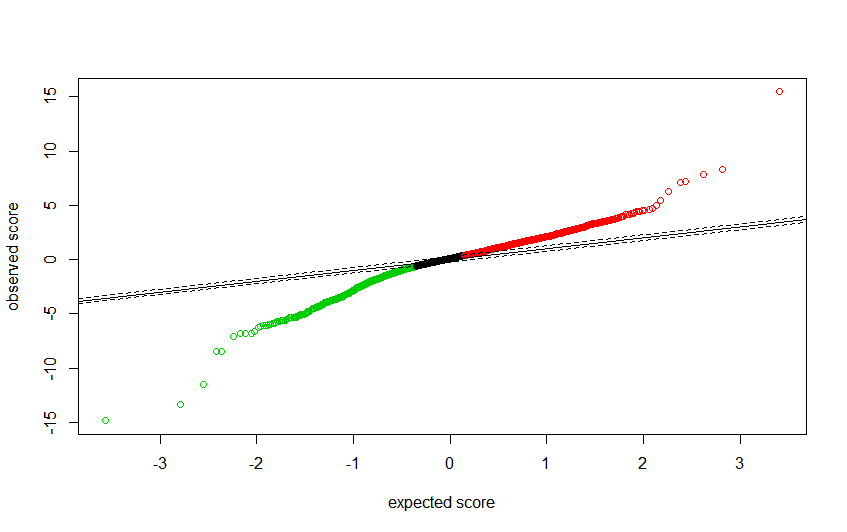
\includegraphics[width=0.7\linewidth]{../ScriptsR/Rplot}
	\caption{Graph of the results of a SAM analysis with parameters fdr.output = 0.2 and nperms = 100 with the first set of rna. The Delta value is 0.24, letting many genes marked as over- or under-expressed. Note: the delta and fold-change parameters are estimated by the SAM function but can be specified by the user.}
	\label{fig:rplot}
\end{figure}
	
	
	
	
\end{enumerate}

\end{document}